\documentclass[11pt]{article}
\usepackage[letterpaper,margin=1in]{geometry}
\usepackage[T1]{fontenc}
\usepackage{amsmath,booktabs,tabularx,enumitem,tikz,natbib,graphicx}
\usetikzlibrary{positioning}
\usepackage[hidelinks]{hyperref}
\title{\textbf{Institutions for Distributed Discovery}\\[0.3em]\large Evidence Acquisition, Adaptation, Coverage, Incentives, and Measurement}
\author{Yohei Nakajima\\Untapped Capital}
\date{July 2026}
\begin{document}\maketitle
\begin{abstract}
Distributed discovery turns evidence into a portfolio of actions. This working
paper organizes completed bounded results by an institutional stack: acquire,
disclose, allocate, adapt, cover, reward, and measure. The taxonomy is an
organizing device, not an empirical theorem. Every numerical statement is tied
to a study claim and immutable run in the public repository.
\end{abstract}
\noindent\textbf{Evidence status.} DD-004--DD-006A are exact bounded computations;
DD-007 is synthetic-only; DD-008 is an exact synthetic source-choice fixture.
No real-institutional claim or peer-review claim is made.
\par\noindent\textbf{Publication status.} Synthesis note; not submitted, not
peer reviewed, and no DOI.
\section{The Discovery Stack}
\begin{center}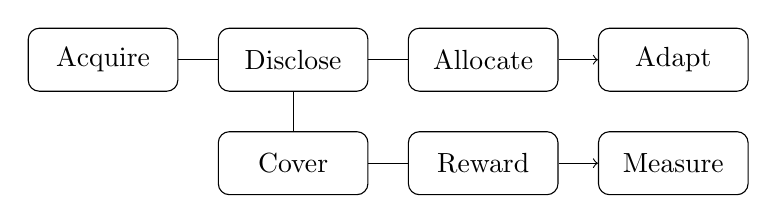
\begin{tikzpicture}[node distance=5mm, every node/.style={draw,rounded corners,align=center,minimum width=19mm,minimum height=8mm}]
\node (a) {Acquire}; \node[right=of a] (d) {Disclose}; \node[right=of d] (l) {Allocate};
\node[right=of l] (ad) {Adapt}; \node[below=of d] (c) {Cover}; \node[right=of c] (r) {Reward}; \node[right=of r] (m) {Measure};
\draw[->] (a)--(d)--(l)--(ad); \draw[->] (d)--(c)--(r)--(m);
\end{tikzpicture}\end{center}
The stack separates margins that are often conflated. Acquisition determines
which signals exist; disclosure determines what becomes shared; allocation maps
information to actions; adaptation uses feedback; coverage evaluates union value;
rewards alter private incentives; measurement determines what can be inferred.
% Generated evidence asset; do not edit by hand.
% Source runs: 20260721T050038Z_DD-004_8ab02e7f_71d84de7c4, 20260721T050706Z_DD-005_be3b544c_98698dee2f, 20260721T140745Z_DD-006_401ad624_c942f43e42, 20260721T052307Z_DD-007_af4ea130_72fb89c5fc, 20260721T141527Z_DD-008_0d11dc77_7e0c8f1d66
\begin{table}[t]\centering\small
\caption{Evidence inventory for the Discovery Stack. Each row is a bounded registered result, not a universal institutional law.}
\label{tab:stack-evidence}
\begin{tabularx}{\textwidth}{lXrr}
\toprule Margin & Registered object & Evidence & Claim\\\midrule
Adapt & 16 schedule records under perfect elimination & exact fixture & DD-C-0045\\
Cover & 3 coverage-frontier records & bounded witnesses & DD-C-0046, DD-C-0047\\
Reward & 123 normalized-transfer rows & exhaustive class & DD-C-0050\\
Acquire & 5 common-source trap cells & exact source-choice grid & DD-C-0051\\
Measure & synthetic event generator and recovery checks & synthetic-only & DD-C-0049\\
\bottomrule\end{tabularx}
\par\footnotesize Generator: \texttt{\detokenize{distributed_discovery.papers.build_discovery_institutions}}; inputs are checksum-validated from immutable manifests.
\end{table}

\section{Evidence discipline}
The stack is deliberately not a single optimization problem. A result at one
margin can be useful while leaving other margins unspecified. The repository
therefore records a claim type, scope statement, immutable manifest, and output
checksums for each finding; aggregation in this paper does not upgrade a claim.
\section{Acquisition}
% Claim: DD-C-0051; run: 20260721T141527Z_DD-008_0d11dc77_7e0c8f1d66
DD-008 compares a free common signal with a costly independent signal in a
two-agent, three-target direct-clue-following fixture. With signal accuracy $p$
and independent-source cost $c$, common/common has social value $p$; one
independent source has $2p-p^2-c$. Private source choice can retain common/common
when one independent source has higher net social value. This is a bounded
accounting result, not a general information-public-good theorem.
The diagnosis is useful because a disappointing portfolio may reflect source
correlation, poor sharing, or convergent actions---three distinct interventions.
This source-choice fixture is adjacent to organizational screening and parallel
search rather than a general theory of either
\citep{SahStiglitz1986,KormanRodeh2020}.
\section{Disclosure and allocation}
DD-001 and DD-002 show that sharing evidence and selecting an action are distinct
operations. Role policies can improve a finite private-information fixture, and
the effect of a disclosure refinement depends on the declared equilibrium
selection rule. These are claim-specific bounded results rather than a
monotonicity failure for all information structures.
Accordingly, planner, pure-equilibrium, and selected-equilibrium quantities are
reported separately rather than collapsed into a claim that ``information helps.''
\section{Adaptation}
% Claim: DD-C-0045; run: 20260721T050038Z_DD-004_8ab02e7f_71d84de7c4
In DD-004's perfect-elimination fixture, batch schedules share terminal discovery
but differ in expected actions and rounds. Thus terminal discovery and operating
cost are distinct objectives; no noisy-test or general adaptivity conclusion
follows.
Terminal discovery and operating cost are thus distinct objectives. A general
sequential design conclusion would require noisy outcomes and a stopping model.
\section{Coverage}
% Claims: DD-C-0046, DD-C-0047; run: 20260721T050706Z_DD-005_be3b544c_98698dee2f
DD-005's finite overlap witnesses show why action labels and individual rankings
are insufficient summaries of portfolio value. The results do not contradict
general approximation guarantees for monotone submodular objectives.
The relevant object is a portfolio, not a list of individually high-scoring
actions; this remains a finite modeling warning, not a universal ranking result.
\section{Rewards}
% Claims: DD-C-0048, DD-C-0050; runs: 20260721T051457Z_DD-006_d49a50ea_068bce4af3, 20260721T140745Z_DD-006_401ad624_c942f43e42
DD-006 separates weak from strict implementation. The score-difference census
and the broader normalized linear frontier both contain weak rows but no strict
truthful/direct implementation under the registered observability and tie rules.
This is not dominant-strategy implementation or an arbitrary-transfer-table
impossibility result.
The normalized linear census leaves nonlinear, contingent, and differently
observable mechanisms open for new registrations.
Potential games, distributed welfare games, and utility design are the closest
general implementation neighbors; the bounded zero-margin result does not
characterize those classes
\citep{MondererShapley1996,MardenWierman2013,PaccagnanChandanMarden2020}.
\section{Measurement}
% Claim: DD-C-0049; run: 20260721T052307Z_DD-007_af4ea130_72fb89c5fc
DD-007 validates synthetic event records and estimator recovery only under its
generator. Matching error creates attenuation and explicit counterexamples show
that action duplication or missing provenance alone need not identify copying or
effective channels.
Measurement is part of the institution: without source and action provenance,
multiple behavioral mechanisms can fit the same aggregate record.
\section{Institutional implications and limitations}
The program supports a design discipline: name the evidence source, the action
portfolio, feedback process, reward observability, and measurement target before
claiming improvement. The studies are small, deliberately registered fixtures.
They do not identify universal institutional laws, analyze real data, or establish
causal effects in organizations.
The synthesis recommends a sequence: name evidence, sharing, allocation,
diversification, feedback, feasible rewards, and measurable outcomes before
claiming an institutional improvement.
\section{Research agenda}
Future work requires new registrations for noisy adaptation, stochastic coverage,
arbitrary transfer tables, richer source-choice games, and any real-data protocol.
\bibliographystyle{plainnat}\bibliography{generated/references}
\end{document}
